To solve this problem, the monitoring region is partitioned into several small rectangles using the proposed Adaptive Partition method. After that, we try to figure out if there is a continuous barrier from the left side to the right side of the region consisting of rectangles which are multiple-view covered. The details are shown in the subsequent sections.

\subsubsection{Multiple-view verification on a rectangle}
\label{subsec:01}
% introduction idea
Based on theorem 2, we can conclude that in order to verify the multiple-view coverage on a rectangle, it is sufficient to check whether all four vertices of that rectangle is multiple-view covered by an common list of sensors. Using this conclusion, we propose an algorithm to verify multiple-view coverage on a rectangle, and for the optimization of the second problem, we try to find the list that multiple-view cover the rectangle with the largest coverage value. 
% 4 steps
%The idea of our algorithm can be described as follows:
The following steps describes the idea to verify if rectangle $ABCD$ is ($k,\omega$) covered:
\begin{description}
	\item[Step 1:] Find a set of sensors $G$ that cover four vertices of the rectangle $ ABCD $.
	\item[Step 2:] Find all lists of $k$ sensors from $G$ satisfies that the point $A$ is ($k,\omega$) covered by these $k$ sensors.
	\item[Step 3:] Among found lists, filter out those which do not simultaneously ($k,\omega$) cover three points $B$, $C$, $D$. This step will offer all lists of sensors that $(k,\omega)$ cover the rectangle $ABCD$. If there does not exist such a list, $ABCD$ is not ($k,\omega$) covered. Otherwise, go to {\bfseries Step 4}.
%	\item[Step 4:] There are 2 possible approaches to choose a single list of sensors in the list of sensor lists found in step 3. These approaches will later be called node handling methods. The maximum method is choosing the list which offers the highest coverage toward the rectangle, while the random one will choose a random list which is expected to give the expectation of all list that $(k-\omega)$ cover the rectangle. In this paper, both approaches are considered and experimented on, detailed result can be found later in section \ref{sec:exp}
	\item[Step 4:] From lists found in {\bfseries Step 3}, select one to later perform coverage quality evaluation on. There are 2 ways to choose the appropriate list among the satisfying lists found, which will later be called node handling method:
	\begin{itemize}
		\item Max method: The chosen list would be the one which offers the greatest coverage value toward the considered node.
		\item Random method: A random list is chosen, this list is expected to reveal the expectation of coverage value of all the sensor lists that $(k-\omega)$ cover the considered node.
	\end{itemize}
\end{description}
\par Note that to verify ($k,\omega$) coverage on $ABCD$, it is sufficient to stop at {\bfseries Step 3}. {\bfseries Step 4} is necessary to perform evaluation of quality coverage on $ABCD$. Criteria for selection in {\bfseries Step 4} is called {\itshape node handling method}. In this paper, we consider two node handling methods, which are the max and the random ones. Different node handling methods are considered to guarantee that our algorithm is convergent and stable in different scenarios. They also contribute to offer alternative options in analysing the $(k-\omega)$ barrier coverage problem (detailed results can be found later in section \ref{sec:exp})\par
The key to implement this idea is at {\bfseries Step 2}. Our approach to this problem is very natural. First, sort $G$ in counter-clockwise order around $A$. Then, we consider each sensor in $G$ sequentially. If the sensor being considered satisfies some conditions, we put it into a list (call this list $L$). We do that until size of $L$ is equal to $k$. Then, $L$ is called a valid list. Figure \ref{finding} illustrates how to choose a valid list. In figure \ref{finding}, black vector denotes the sensor that is chosen to put into the list, while red vector denotes candidates to be chosen.

\begin{figure}[!h]
	\begin{minipage}{.3\linewidth}
		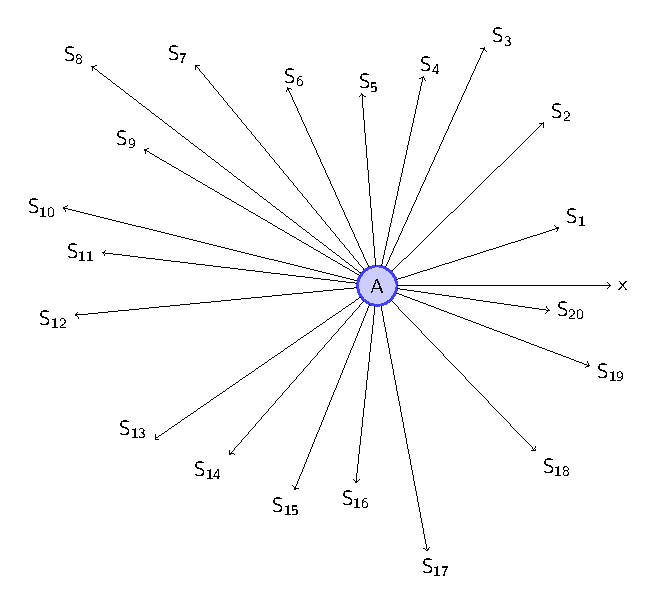
\includegraphics[scale=.5]{setSensors_1.pdf}
	\end{minipage}
	\hfill
	\begin{minipage}{.3\linewidth}
		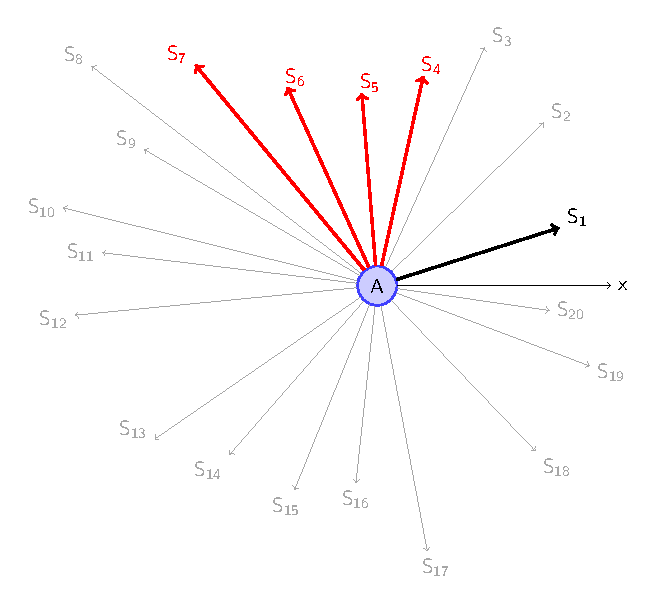
\includegraphics[scale=.5]{setSensors_2.pdf}
	\end{minipage}
	\hfill
	\begin{minipage}{.3\linewidth}
		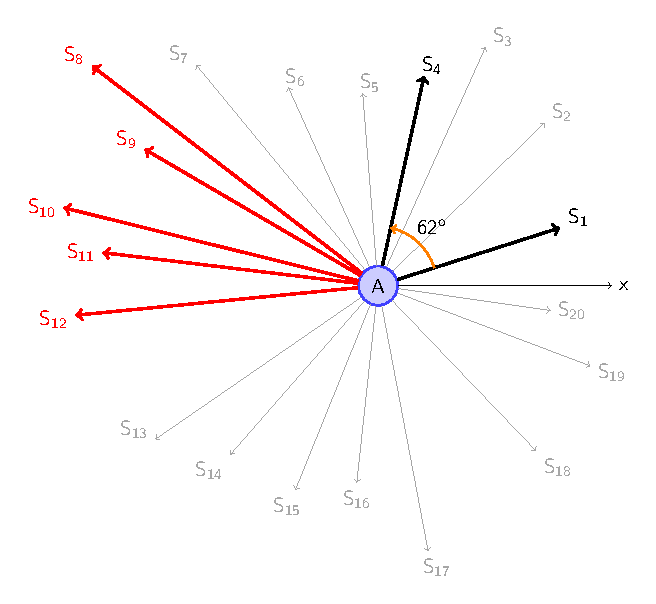
\includegraphics[scale=.5]{setSensors_3.pdf}
	\end{minipage}
	\\
	\begin{minipage}{.3\linewidth}
		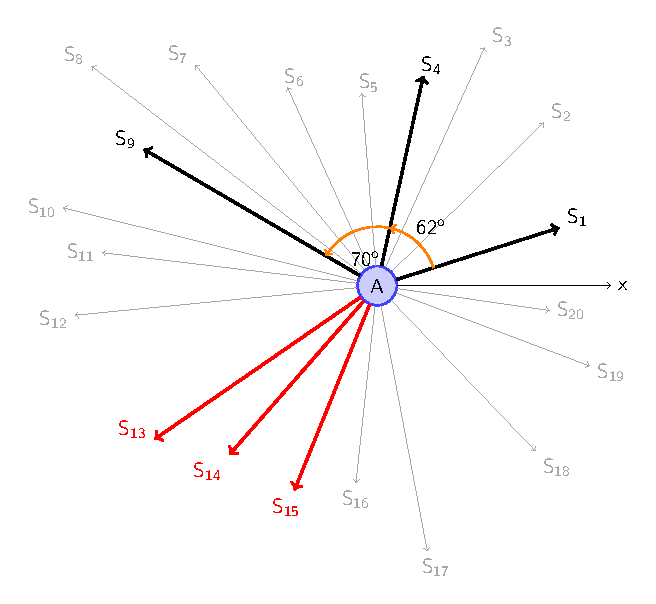
\includegraphics[scale=.5]{setSensors_4.pdf}
	\end{minipage}
	\hfill
	\begin{minipage}{.3\linewidth}
		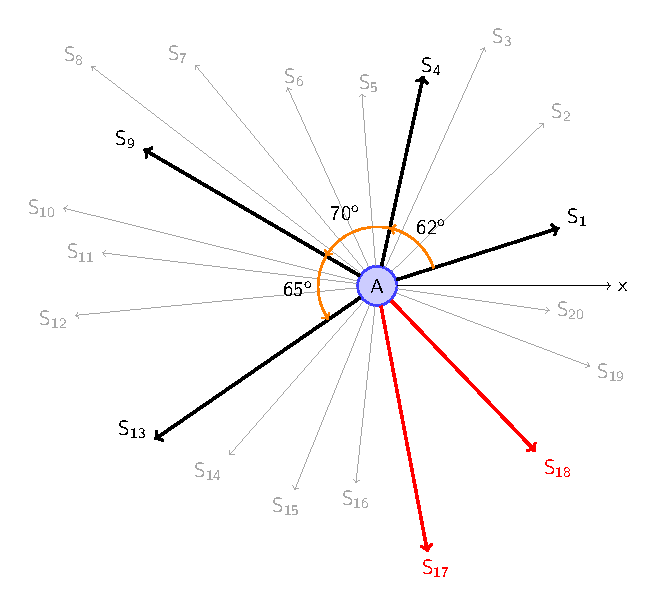
\includegraphics[scale=.5]{setSensors_5.pdf}
	\end{minipage}
	\hfill
	\begin{minipage}{.3\linewidth}
		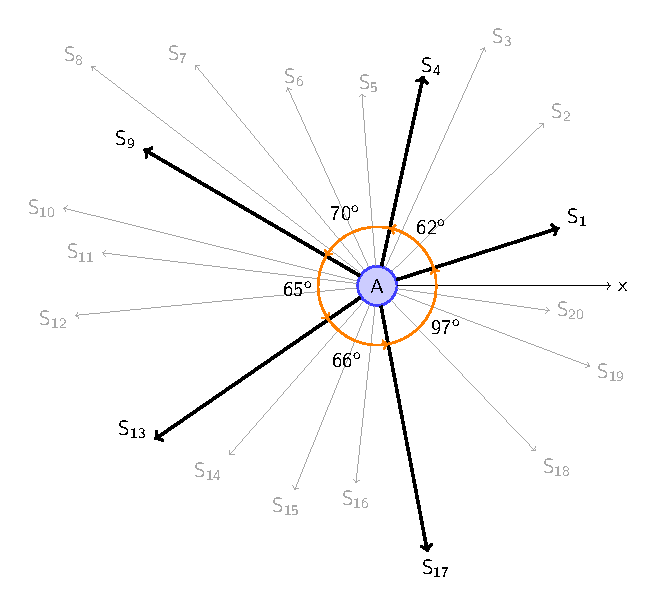
\includegraphics[scale=.5]{setSensors_6.pdf}
	\end{minipage}\\
	\caption{$L=\{S_1, S_4, S_9, S_{13}, S_{17}\}$ is a valid list with $k=5, \omega=60^o$}
	\label{finding}
\end{figure}

As aforementioned, when considering a sensor in $G$, it must satisfies some conditions to become candidate to be put into the list $L$. Suppose that at some point of the finding process, the list has {\sf\itshape index} elements and {\sf\itshape $L$[index] = $G$[current]}, {\sf\itshape 1} $\leq$ {\sf\itshape current} $\leq$ {\sf\itshape $n$}, $n$ is size of $G$. If {\sf\itshape $G$[next]} is chosen to be the next element in $L$, it must satisfy two conditions:
\begin{itemize}
	\item $(\overrightarrow{\vphantom{\overrightarrow{P}}PG\textsf{[cur]}}, \overrightarrow{\vphantom{\overrightarrow{P}}PG\textsf{[next]}}) > \omega \qquad (i)$
	\item $(\overrightarrow{\vphantom{\overrightarrow{P}}PG\textsf{[next]}}, \overrightarrow{\vphantom{\overrightarrow{P}}PL\textsf{[1]}}) > (k-\textsf{index})\omega \qquad (ii)$
\end{itemize}
From definition of ($k,\omega$) coverage, condition (i) is clearly necessary. However, it's not sufficient for {\sf\itshape $G$[next]} to become a candidate for the next position in $L$. If $L$ is a valid list, we have $(\overrightarrow{\vphantom{\overrightarrow{P}}PL[i]}, \overrightarrow{\vphantom{\overrightarrow{P}}PL[i+1]}) > \omega, i = \overline{1,k}$ (consider $k + 1 = 1$). Hence, $(\overrightarrow{\vphantom{\overrightarrow{P}}PL\textsf{[index + 1]}}, \overrightarrow{\vphantom{\overrightarrow{P}}PL[1]}) = \displaystyle\sum\limits_{i=\textsf{\scriptsize index} + 1}^{k}(\overrightarrow{\vphantom{\overrightarrow{P}}PL[i]}, \overrightarrow{\vphantom{\overrightarrow{P}}PL[i+1]}) > (k-\textsf{index})\omega$.
Since we are choosing candidate for {\sf (index + 1)-th} element in $L$, {\sf $G$[next]} corresponds to {\sf $L$[index + 1]}. Thus, (ii) is also a necessary condition.\\[7pt]
Algorithm \ref{alg00} and \ref{alg01} show the details of our method. Algorithm \ref{alg01} is a support function for Algorithm \ref{alg00}. {\tt RecurFinding(cur)} is a recursive function that finds candidate for {\sf (index + 1)-th} position in $L$ knowing that there is a set {\sf cur} containing the chosen sensors, in which the last sensor has index {\sf last}. It considers elements in $G$ sequentially from {\sf (last + 1)-th} element and checks if these elements satisfy condition (i) and (ii). The return value of {\tt RecurFinding(cur)} is a set containing all the lists of sensors that ($k-\omega$) cover the point $P$ which takes the current sublist ($\{L\textsf{[1]}, L\textsf{[1]},..., L\textsf{[index]}\}$) as its first {\sf index} elements exists. This return value is used to support the recursion process of the algorithm.

\noindent\begin{minipage}{.49\linewidth}
	\begin{algorithm}[H]
		\DontPrintSemicolon 
		\SetAlgoLined
		\newcommand{\forcondi}[2]{\ensuremath{#1 \in #2}}
		\SetKwData{found}{found}
		\SetKwData{Gsize}{G.size}
		\SetKw{true}{true}
		\SetKw{false}{false}
		\SetKwData{and}{\&\&}
		\SetKwData{equal}{==}
		\SetKwData{greater}{$\geq$}
		\SetKwData{notFound}{!found}
		\SetKwData{k}{k}
		\SetKwData{n}{n}
		\newcommand{\forcond}[3]{\ensuremath{#1 = #2\ \KwTo\ #3}}
		\BlankLine
		\KwIn{
			A point {\sf P} and a set {\sf G} consisting of {\sf n} sensors that cover {\sf P}.
		}
		\KwOut{
			\k sensors that ($\mathsf{k-\omega}$) covers {\sf P}. There is possibility that no output is found.
		}
		\BlankLine
		\BlankLine
		Let {\sf L} store the output\;
		Sort {\sf G} in counter-clockwise order around {\sf P}\;
		$L \leftarrow \emptyset$\;
		\For{\forcond{i}{1}{n}}{
			$temp \leftarrow {\tt RecurFinding(G{i})}$\;
			$L \leftarrow L \cup temp$\;
		}
		\caption{Find all lists of $k$ sensors that ({\sf $k-\omega$}) covers point $P$}
		\label{alg00}
	\end{algorithm}
\end{minipage}
\hfill
\begin{minipage}{.49\linewidth}
	\begin{algorithm}[H]
		\DontPrintSemicolon
		%	\SetAlgoNoLine
		%	\SetAlgoNoEnd
		\newcommand{\forcondi}[2]{\ensuremath{#1 \in #2}}
		\SetKwData{found}{found}
		\SetKwData{Gsize}{G.size}
		\SetKw{true}{true}
		\SetKw{false}{false}
		\SetKwData{and}{\&\&}
		\SetKwData{equal}{==}
		\SetKwData{greater}{$\geq$}
		\SetKwData{notFound}{!found}
		\SetKwData{k}{k}
		\SetKwData{n}{n}
		\SetKwData{cur}{cur}
		\SetKwArray{G}{G}
		\SetKwArray{L}{L}
		\SetKwData{P}{P}
		\SetKwFunction{Recur}{RecurFinding}
		\SetKwData{paratwo}{\tt index + 2, i}
		\SetKwData{paraone}{index + 1}
		\SetKwData{index}{index}
		\SetKw{return}{return}
		\SetKwProg{Fn}{}{}{end}
		\newcommand{\forcond}[3]{\ensuremath{#1 = #2\ \KwTo\ #3}}
		\BlankLine
		\KwIn{
			A list of sensors that is currently chosen, contains \index sensors.
		}
		\KwOut{
			All lists of \k sensors that ($k-\omega$) cover the point \sf P beginning with the input list.
		}
		\BlankLine
		\BlankLine
		\Fn{\tt RecurFinding({\sf cur})}{
			$L \leftarrow \emptyset$\;
			$\index \leftarrow$ cardinality of {\sf cur}\;
			\If{m \equal k}{\return {\sf \{cur\}}}
			$last \leftarrow$ index of last element in {\sf cur}\; 
			$first \leftarrow$ index of first element in {\sf cur}\;
			\For{\forcond{i}{last + 1}{\n}}{
				\If{
					$(\overrightarrow{\vphantom{\overrightarrow{P}} \P\G{last}}, \overrightarrow{\vphantom{\overrightarrow{P}} \P\G{i}}) > \omega$ \and
					$(\overrightarrow{\vphantom{\overrightarrow{P}} \P\G{i}}, \overrightarrow{\vphantom{\overrightarrow{P}} \P\G{first}}) > (\k - \index + 1)\omega$
				}{
					$temp \leftarrow$ {\tt RecurFinding({\sf cur} + (\G{i}))}\;
					$L \leftarrow L \cup temp$\;
				}
			}
			\return L\;
		}
		\caption{Find {\sf index + 1} element in {\sf L}}
		\label{alg01}
	\end{algorithm}
\end{minipage}

%\begin{figure*}[!h]
%\noindent\begin{minipage}{.49\linewidth}
%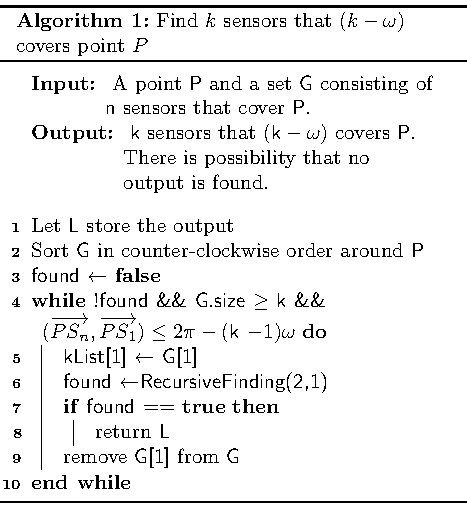
\includegraphics{Algo_1.pdf}
%\end{minipage}\hfill
%\begin{minipage}{.49\linewidth}
%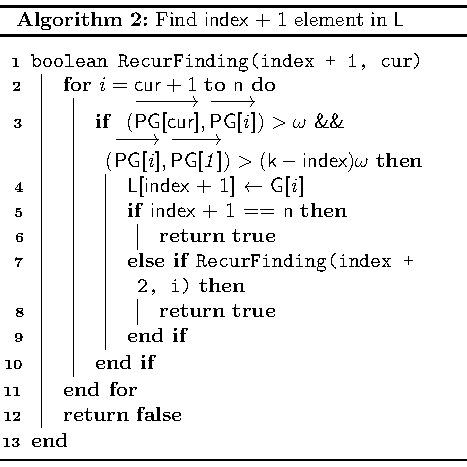
\includegraphics{Algo_2.pdf}
%\end{minipage}
%\end{figure*}

The first element of $L$ can be any sensor in $G$ since it doesn't require any condition. For convenient, we choose $L[1]=G[1]$. Thus, {\tt RecurFinding(\{G[1]\})} is called to start the finding process. After function call {\tt RecurFinding(\{G[1]\})}, the function will return all the satisfied lists containing G[1]. The finding process stops when we have called {\tt RecurFinding(\{G[$i$]\})} with every $i$ from 1 to n. And the algorithm will output a set containing all the lists of sensors that ($k-\omega$) cover the considered point $P$.

\subsubsection{Finding a barrier in a monitoring region}


a, Partitioning the monitoring region by Adaptive Partition method

\label{subsection1}

To find a barrier in the monitoring region, we first determine the areas that are multiple-view covered inside the region of interest $\Omega$. To solve this problem, we partition $\Omega$ into multiple small rectangles and check whether these rectangles are multiple-view covered or not. However, uniform partitioning often requires a high computation time especially when the $\Omega$ is large. To overcome this challenge, we propose a new partition method called Adaptive Partition. The idea of the Adaptive Partition method is as follows: only the rectangles which are not multiple-view covered will be partitioned into smaller rectangles, otherwise, they are kept untouched. \par
The first rectangle to be checked is the monitoring region. 
Using the algorithm in \ref{subsec:01}, if a rectangle is multiple-view covered, mark it as true, otherwise, split it into four equal sub-rectangles. After a rectangle is split, smaller rectangles are generated and the process of checking and splitting is applied to these new rectangles. A rectangle will not be split if it is multiple-view covered or its size reaches a predefined limited value. The smaller the limited size is, the more precise the result of our algorithm can get. This condition guarantees our algorithm not to go into an infinite loop. The process is illustrated in Figure \ref{dynamic}.
%\input{DynamicPartition}
\begin{figure}[!h]
	\begin{center}
		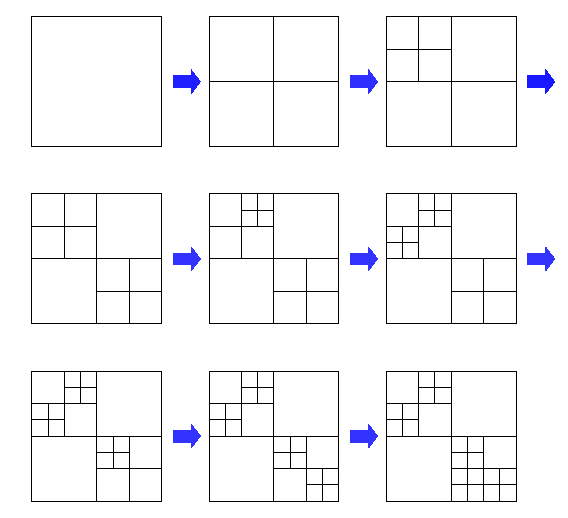
\includegraphics[scale=1.]{Dynamic_Partition.pdf}
	\end{center}
	\caption{Illustration of Adaptive Partitioning}
	\label{dynamic}
\end{figure}

The pseudo code of the method is described in Algorithm \ref{alg3}
%

%
\begin{center}
	\begin{minipage}{.7\linewidth}
		\begin{algorithm}[H]
			\DontPrintSemicolon
			\SetAlgoLined
			\newcommand{\forcondi}[2]{\ensuremath{#1 \in #2}}
			\SetKwData{Rcen}{root.center}
			\SetKwData{root}{rootRec}
			\SetKwData{RX}{root.sizeX}\SetKwData{RY}{root.sizeY}
			\SetKwData{L}{L}\SetKwData{W}{W}
			\SetKwData{QUEUE}{Q}
			\SetKwData{tempNode}{tempRec}
			\SetKwData{coveredGroup}{coveredGroup}
			\SetKwFunction{FAC}{findAndCheck}
			\SetKwData{coveredNodes}{coveredRectangles}
			\SetKwData{DMAX}{DMAX}
			\SetKwFunction{split}{split()}
			\SetKwFunction{makeNode}{makeNode}
			\SetKwFunction{dequeue}{dequeue}
			\SetKwFunction{enqueue}{enqueue}
			\SetKwFunction{check}{check}
			\SetKwData{tnRank}{tempRec.rank}
			\SetKwData{element}{element}
			\BlankLine
			\KwIn{
				\begin{itemize}
					\item \L, \W: Length and width of the monitoring region $\Omega$ respectively
					\item A set of deployed sensors $S$
					\item Minimum size of a grid
				\end{itemize}
			}
			\KwOut{A set of multiple-view covered rectangles $\Pi$}
			\BlankLine
			\BlankLine
%			Let \coveredNodes store the output\;
			Let \root denote the monitoring region\;
			$\QUEUE\gets$ \O \;
			\enqueue{\root, \QUEUE} \;
			\While{$\QUEUE \neq$ \O}{
				$\tempNode\gets$ \dequeue{\QUEUE}\;
%				Check if \tempNode is $(k-\omega)$ covered\;
				\uIf{\tempNode is multiple-view covered}{add \tempNode to $\Pi$\;}
				\ElseIf{\tempNode has not reached the minimum size}{split \tempNode into 4 sub-rectangles\;
					add 4 sub-rectangles of \tempNode to \QUEUE}
			}
			\caption{Adaptive Partition}
			\label{alg3}
		\end{algorithm}
	\end{minipage}
\end{center}

b, Finding a multiple-view coverage barrier

After procedure in \ref{subsec:01}, we now have a set $\Pi$ of rectangles that are multiple-view covered. To find a multiple-view covered barrier, we need to find a continuous area formed from rectangles in $\Pi$ that connects the left side to the right side of $\Omega$. The method is to transform the rectangles set into a graph. Each vertex in the graph corresponds to a rectangle in $\Pi$. Two vertices are considered adjacent if the corresponding rectangles share at least one point. Two virtual vertices are added to the graph, source vertex {\tt source} and sink vertex {\tt sink}. All vertices corresponding to the rectangles lying on the left side of $\Omega$ are adjacent to {\tt source} and all vertices corresponding to the rectangles lying on the right side of $\Omega$ are adjacent to {\tt sink}. After constructing the graph, we use Breath First Search algorithm to find a path from {\tt source} to {\tt sink}. If a path is found, we conclude that there exists a multiple-view barrier in the monitoring region. Otherwise, the barrier does not exist.